\chapter{Studio di funzione}
\texttt{In analisi matematica la locuzione studio di funzione indica 
	l'applicazione pratica dei teoremi e delle tecniche del calcolo 
	infinitesimale nello specifico caso di una funzione di cui è nota 
	l'espressione analitica. Lo studio di funzione è utile per ricavare 
	esplicitamente le informazioni che descrivono il comportamento di una 
	funzione nel suo dominio. Spesso, le informazioni ottenute mediante uno 
	studio di funzione sono sufficienti per poter tracciare, anche a mano, un 
	grafico qualitativo della funzione studiata e che in genere, per funzioni a 
	valori reali di una variabile reale, viene rappresentato su un piano 
	cartesiano, anche se in taluni casi potrebbe essere più semplice ricorrere 
	un sistema di coordinate differente. In genere, con "studio di funzione" ci 
	si riferisce implicitamente al solo e specifico caso delle funzioni reali di
	una sola variabile reale, ma con le opportune modifiche è comunque possibile 
	adattare le considerazioni seguenti anche al caso delle funzioni di più
	variabili reali, nonché anche per le funzioni di una o più variabili 
	complesse.}
\begin{center}
	By \href{https://it.wikipedia.org/wiki/Studio_di_funzione}{Wikipedia}
\end{center}

\section{Grafica delle funzioni elementari}
\subsection{Funzione lineare $y=mx+qm, q\in R$}
\begin{figure}[!ht]
	\centering
	\begin{tikzpicture}
		\node[] (pic) at (0,0) {\includegraphics[height=8cm]{img/funzione
		lineare.pdf}};
	\end{tikzpicture}
	\caption{Grafico di Funzione lineare $y=mx+qm, q\in R$}
\end{figure}
$C.E. \equiv R\text{ Non Limitata}$
\subsection{Funzione valore assoluto $y=|x|$}
\begin{figure}[!ht]
	\centering
	\begin{tikzpicture}
		\node[] (pic) at (0,0) {\includegraphics[height=8cm]{img/funzione valore assoluto.pdf}};
	\end{tikzpicture}
	\caption{Grafico di Funzione valore assoluto $y=|x|$}
\end{figure}
$C.E. \equiv R\text{ Limitata inferiormente in } x=0$\\
$|x|=\begin{cases}
	x&x\geq0\\
	-x& x<0
\end{cases}$
\subsection{Funzione potenza $y=x^n,n\in N, pari$}
\begin{figure}[!ht]
	\centering
	\begin{tikzpicture}
		\node[] (pic) at (0,0) {\includegraphics[height=8cm]{img/funzione
		potenziale x^n.pdf}};
	\end{tikzpicture}
	\caption{Grafico di Funzione potenza $y=x^n,n\in N, pari$}
\end{figure}\newpage
\subsection{Funzione potenza $y=x^\alpha,\alpha \in R$ (\textit{ma non
razionale})}
\begin{figure}[!ht]
	\centering
	\begin{tikzpicture}
		\node[] (pic) at (0,0) {\includegraphics[height=8cm]{img/funzione
		potenziale x^a.pdf}};
	\end{tikzpicture}
	\caption{Grafico di Funzione potenza $y=x^\alpha,\alpha \in R$ (\textit{ma non
razionale})}
\end{figure}
$C.E.:\{x\in R: x\geq 0\}$ Limitata inferiormente da $x=0$ non limitata
superiormente Strettamente crescente
\subsection{Funzione potenziale $y=x^{\frac{m}{n}},m, n\in Z$}
\begin{figure}[!ht]
	\centering
	\begin{tikzpicture}
		\node[] (pic) at (0,0) {\includegraphics[height=8cm]{img/funzione
		potenziale fratta.pdf}};
	\end{tikzpicture}
	\caption{Grafico di Funzione potenza $y=x^\alpha,\alpha \in R$ (\textit{ma non
razionale})}
\end{figure}
\subsection{Funzione logaritmo $y=\log_a{x}$}
\begin{figure}[!ht]
	\centering
	\begin{tikzpicture}
		\node[] (pic) at (0,0) {\includegraphics[height=8cm]{img/funzione
		logaritmica.pdf}};
	\end{tikzpicture}
	\caption{Funzione logaritmo $y=\log_a{x}$}
\end{figure}
$C.E.\equiv x>0$ Non limitata, strettamente crescente se $a>1$, Strettamente
decrescente se $0<a<1$.\newpage
\subsection{Le coniche: la circonferenza}
\begin{figure}[!ht]
	\centering
	\begin{tikzpicture}
		\node[] (pic) at (0,0) {\includegraphics[height=8cm]{img/le coniche
		circonferenze.pdf}};
	\end{tikzpicture}
	\caption{Le coniche: la circonferenza}
\end{figure}\newpage
\subsection{Le coniche: l'ellisse}
\begin{figure}[!ht]
	\centering
	\begin{tikzpicture}
		\node[] (pic) at (0,0) {\includegraphics[height=8cm]{img/le coniche
		ellisse.pdf}};
	\end{tikzpicture}
	\caption{Le coniche: l'ellisse}
\end{figure}
\subsection{Le coniche: iperbole}
\begin{figure}[!ht]
	\centering
	\begin{tikzpicture}
		\node[] (pic) at (0,0) {\includegraphics[height=8cm]{img/le coniche
		iperbole.pdf}};
	\end{tikzpicture}
	\caption{Le coniche: iperbole}
\end{figure}\newpage
\subsection{Le coniche: iperbole equilattera}
\begin{figure}[!ht]
	\centering
	\begin{tikzpicture}
		\node[] (pic) at (0,0) {\includegraphics[height=8cm]{img/le coniche
		iperbole equilattera.pdf}};
	\end{tikzpicture}
	\caption{Le coniche: iperbole equilattera}
\end{figure}
\subsection{Le coniche: parabola}
\begin{figure}[!ht]
	\centering
	\begin{tikzpicture}
		\node[] (pic) at (0,0) {\includegraphics[height=8cm]{img/le coniche
		parabola.pdf}};
	\end{tikzpicture}
	\caption{Le coniche: parabola}
\end{figure}\newpage
\subsection{Le funzioni trigonometriche}
Funzioni trigonometriche elementati:
$y=\sin x, y=cos x, y=\tan x, y=\cot x$\\
\textit{Relazioni fondamentali:} $(\sin x)^2+(\cos x)^2=1$, $\tan x=\frac{\sin
x}{\cos x}$, $\cot x=\frac{\cos x}{\sin x}$
\begin{figure}[!ht]
	\centering
	\begin{tikzpicture}
		\node[] (pic) at (0,0) {\includegraphics[height=8cm]{img/funzioni
		trigonometriche.pdf}};
	\end{tikzpicture}
	\caption{Le funzioni trigonometriche}
\end{figure}
\subsubsection{Funzione $\sin x$}
\begin{figure}[!ht]
	\centering
	\begin{tikzpicture}
		\node[] (pic) at (0,0) {\includegraphics[height=8cm]{img/funzione
		sin.pdf}};
	\end{tikzpicture}
	\caption{Funzione $\sin x$}
\end{figure}\newpage
\subsubsection{Funzione $\cos x$}
\begin{figure}[!ht]
	\centering
	\begin{tikzpicture}
		\node[] (pic) at (0,0) {\includegraphics[height=8cm]{img/funzione
		cos.pdf}};
	\end{tikzpicture}
	\caption{Funzione $\cos x$}
\end{figure}
\subsubsection{Funzione $\tan x$}
\begin{figure}[!ht]
	\centering
	\begin{tikzpicture}
		\node[] (pic) at (0,0) {\includegraphics[height=8cm]{img/funzione
		tg.pdf}};
	\end{tikzpicture}
	\caption{Funzione $\tan x$}
\end{figure}\newpage
\subsubsection{Funzione $\cot x$}
\begin{figure}[!ht]
	\centering
	\begin{tikzpicture}
		\node[] (pic) at (0,0) {\includegraphics[height=8cm]{img/funzione
		ctg.pdf}};
	\end{tikzpicture}
	\caption{Funzione $\cot x$}
\end{figure}
\subsection{Le funzioni trigonometriche inverse}
\subsubsection{Funzione $\arcsin x$}
\begin{figure}[!ht]
	\centering
	\begin{tikzpicture}
		\node[] (pic) at (0,0) {\includegraphics[height=8cm]{img/funzione
		arcsin.pdf}};
	\end{tikzpicture}
	\caption{Funzione $\arcsin x$}
\end{figure}\newpage
\subsubsection{Funzione $\arccos x$}
\begin{figure}[!ht]
	\centering
	\begin{tikzpicture}
		\node[] (pic) at (0,0) {\includegraphics[height=8cm]{img/funzione
		arccos.pdf}};
	\end{tikzpicture}
	\caption{Funzione $\arccos x$}
\end{figure}
\subsubsection{Funzione $\arctan x$}
\begin{figure}[!ht]
	\centering
	\begin{tikzpicture}
		\node[] (pic) at (0,0) {\includegraphics[height=8cm]{img/funzione
		arctg.pdf}};
	\end{tikzpicture}
	\caption{Funzione $\arctan x$}
\end{figure}\newpage
\subsubsection{Operazione sul grafico: traslazione della asse X}
\begin{figure}[!ht]
	\centering
	\begin{tikzpicture}
		\node[] (pic) at (0,0) {\includegraphics[height=8cm]{img/operazione sul
		grafico traslazione della asse x.pdf}};
	\end{tikzpicture}
	\caption{Operazione sul grafico: traslazione della asse X}
\end{figure}
\subsubsection{Operazione sul grafico: traslazione della asse Y}
\begin{figure}[!ht]
	\centering
	\begin{tikzpicture}
		\node[] (pic) at (0,0) {\includegraphics[height=8cm]{img/operazione sul
		grafico traslazione della asse y.pdf}};
	\end{tikzpicture}
	\caption{Operazione sul grafico: traslazione della asse Y}
\end{figure}\newpage
\subsubsection{Operazione sul grafico: contrazione e dilatazione in direzione verticale}
\begin{figure}[!ht]
	\centering
	\begin{tikzpicture}
		\node[] (pic) at (0,0) {\includegraphics[height=8cm]{img/contrazione e
		dilatazione in direzione verticale.pdf}};
	\end{tikzpicture}
	\caption{Operazione sul grafico: contrazione e dilatazione in direzione verticale}
\end{figure}
\subsubsection{Operazione sul grafico: contrazione e dilatazione in direzione
orizzontale}
\begin{figure}[!ht]
	\centering
	\begin{tikzpicture}
		\node[] (pic) at (0,0) {\includegraphics[height=8cm]{img/compressione e
		dilatazione in direzione orizzontale.pdf}};
	\end{tikzpicture}
	\caption{Operazione sul grafico: contrazione e dilatazione in direzione
	orizzontale}
\end{figure}\newpage
\subsubsection{Operazione sul grafico: $y=|f(x)|$}
\begin{figure}[!ht]
	\centering
	\begin{tikzpicture}
		\node[] (pic) at (0,0) {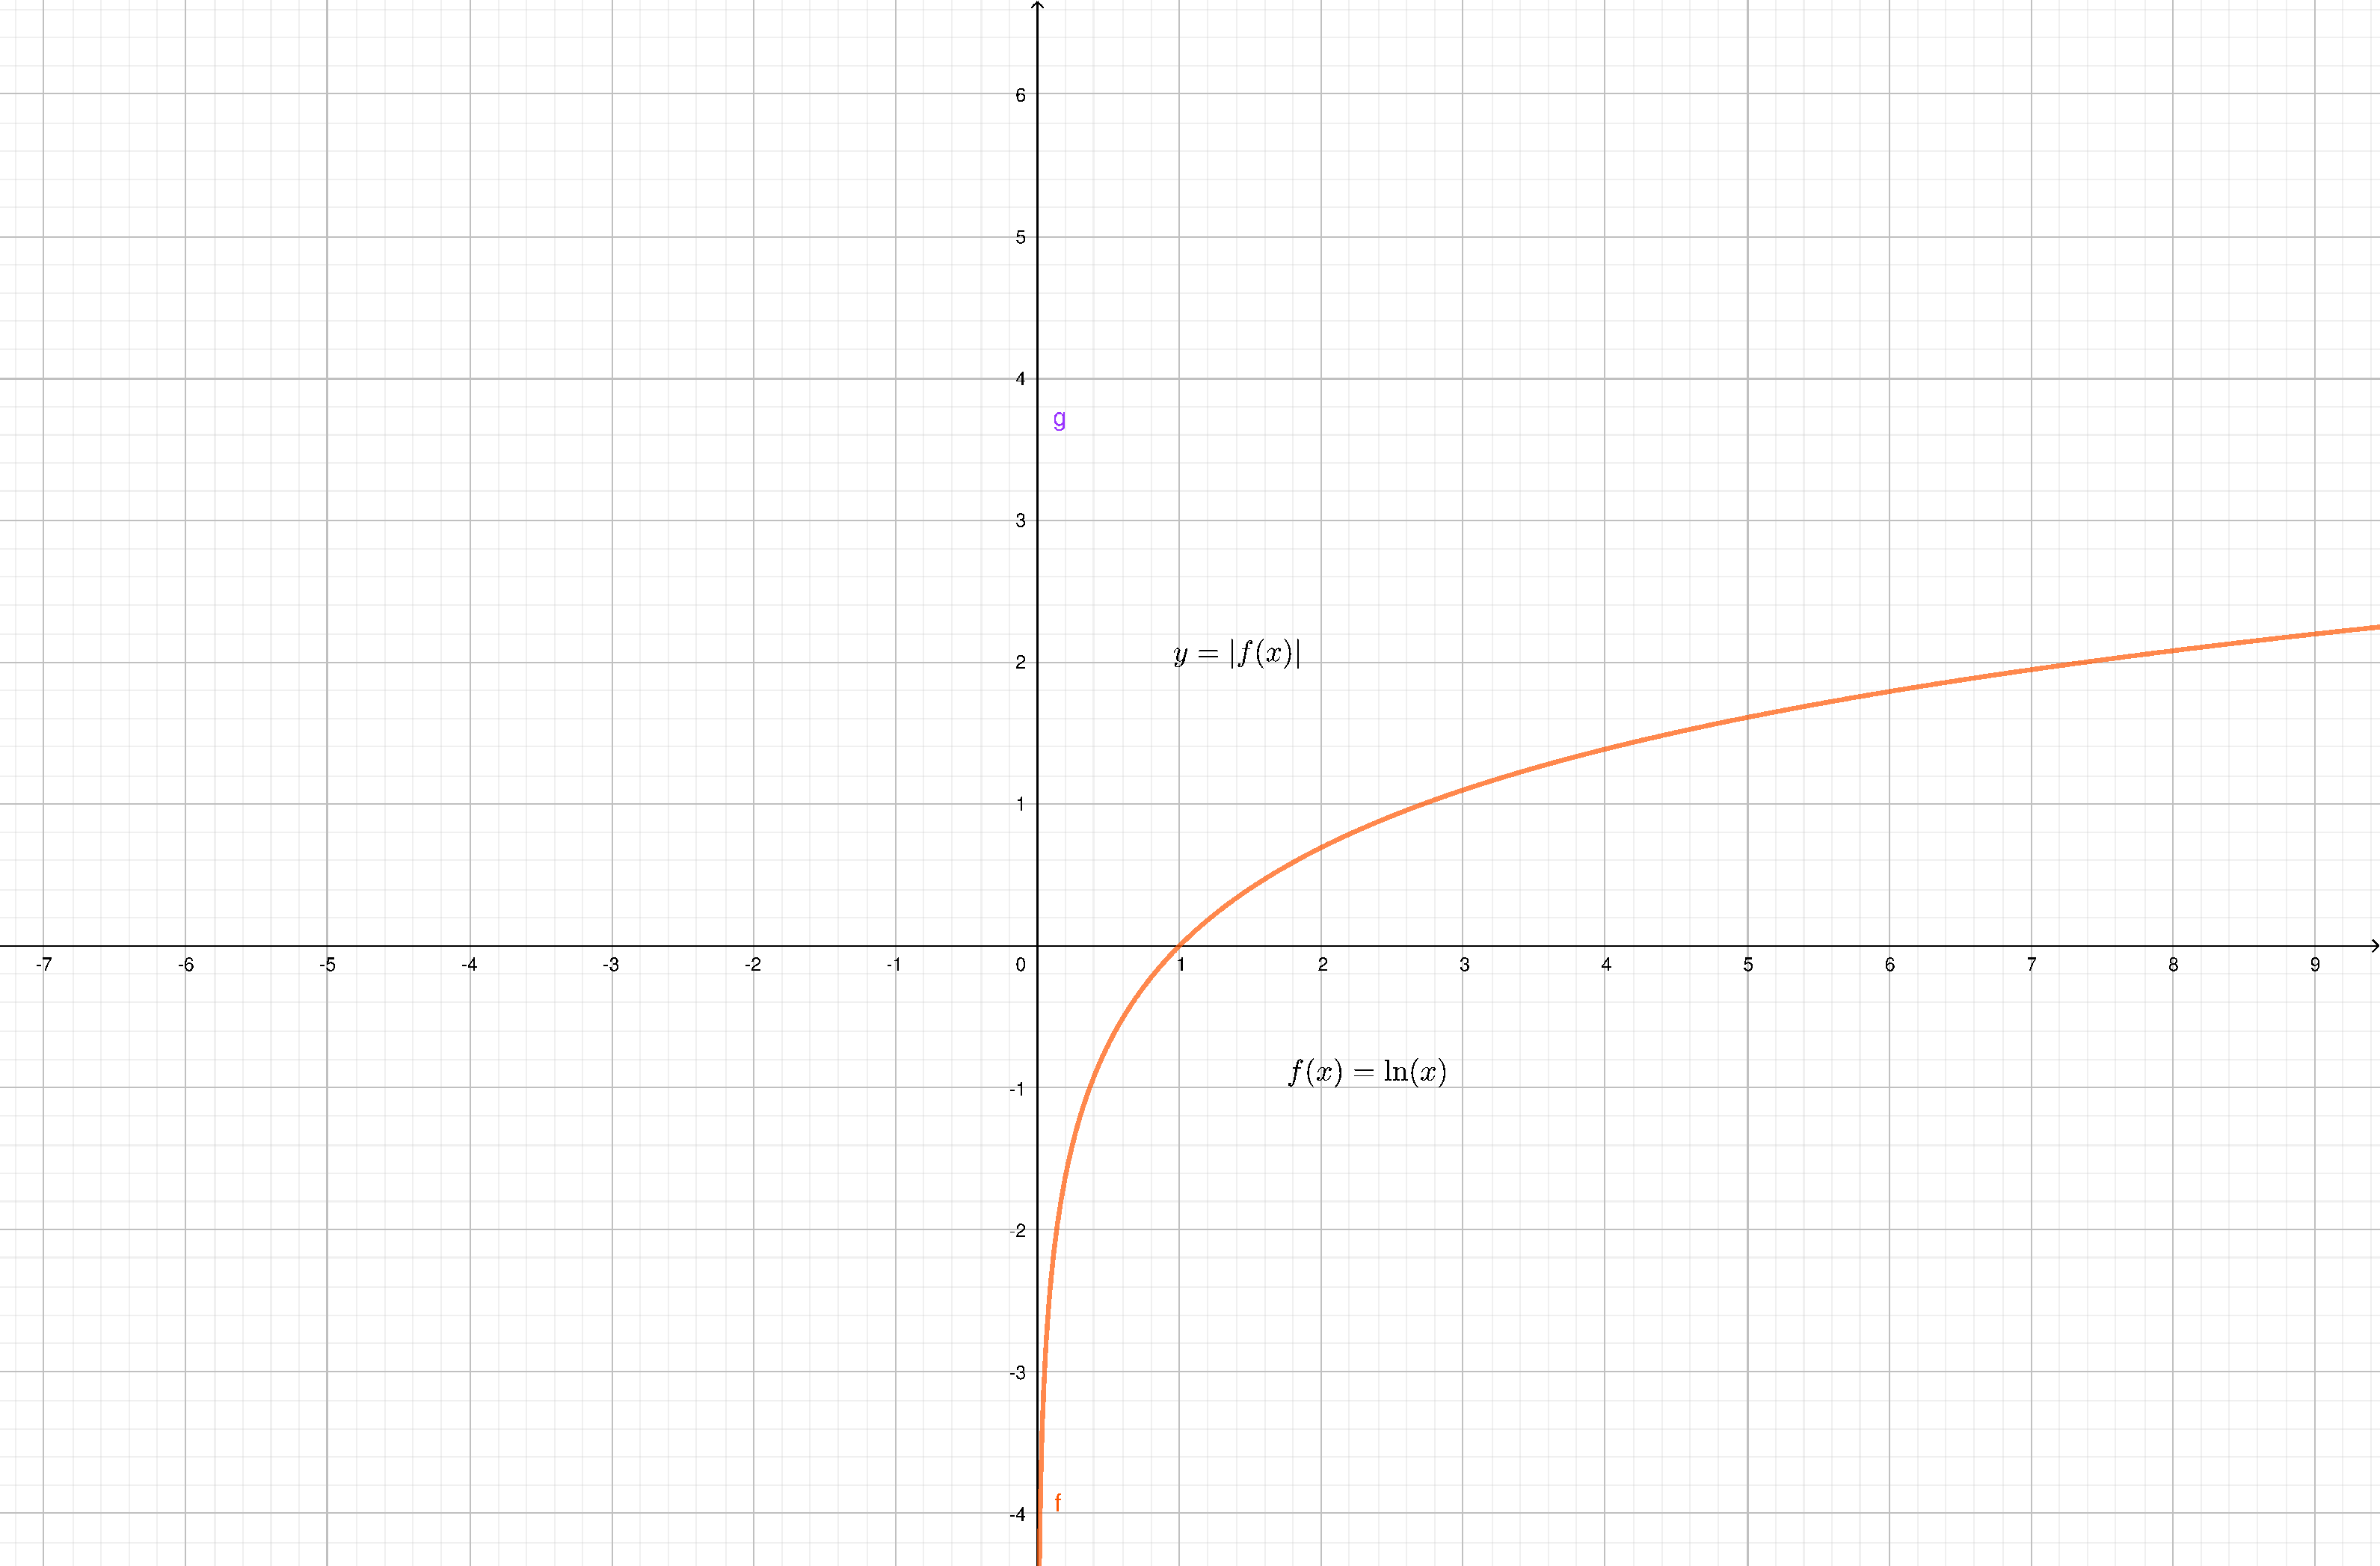
\includegraphics[height=8cm]{img/y=_lnx_.pdf}};
	\end{tikzpicture}
	\caption{Operazione sul grafico: $y=|f(x)|$}
\end{figure}


